\documentclass[11pt,addpoints,answers]{exam}
%\documentclass[11pt]{article}
\usepackage[margin=1in]{geometry}
\usepackage{amsmath, amsfonts}
\usepackage{enumerate}
\usepackage{graphicx}
\usepackage{titling}
\usepackage{url}
\usepackage{xfrac}
% \usepackage{fancyhdr} % CONFLICTS with the exam class
\usepackage{geometry}
\usepackage{graphicx}
\usepackage{natbib}
\usepackage{amsmath}
\usepackage{amssymb}
\usepackage{amsthm}
\usepackage{paralist}
\usepackage{epstopdf}
\usepackage{tabularx}
\usepackage{longtable}
\usepackage{multirow}
\usepackage{multicol}
\usepackage[colorlinks=true,urlcolor=blue]{hyperref}
\usepackage{fancyvrb}
\usepackage{algorithm}
\usepackage{algorithmic}
\usepackage{float}
\usepackage{paralist}
\usepackage[svgname]{xcolor}
\usepackage{enumerate}
\usepackage{array}
\usepackage{times}
\usepackage{url}
\usepackage{comment}
\usepackage{environ}
\usepackage{times}
\usepackage{textcomp}
\usepackage{caption}
\usepackage[colorlinks=true,urlcolor=blue]{hyperref}
\usepackage{listings}
\usepackage{parskip} % For NIPS style paragraphs.
\usepackage[compact]{titlesec} % Less whitespace around titles
\usepackage[inline]{enumitem} % For inline enumerate* and itemize*
\usepackage{datetime}
\usepackage{comment}
% \usepackage{minted}
\usepackage{lastpage}
\usepackage{color}
\usepackage{xcolor}
\usepackage{listings}
\usepackage{tikz}
\usetikzlibrary{shapes,decorations,bayesnet}
%\usepackage{framed}
\usepackage{booktabs}
\usepackage{cprotect}
\usepackage{xcolor}
\usepackage{verbatimbox}
\usepackage[many]{tcolorbox}
\usepackage{cancel}
\usepackage{wasysym}
\usepackage{mdframed}
\usepackage{subcaption}
\usetikzlibrary{shapes.geometric}

%%%%%%%%%%%%%%%%%%%%%%%%%%%%%%%%%%%%%%%%%%%
% Formatting for \CorrectChoice of "exam" %
%%%%%%%%%%%%%%%%%%%%%%%%%%%%%%%%%%%%%%%%%%%

\CorrectChoiceEmphasis{}
\checkedchar{\blackcircle}

%%%%%%%%%%%%%%%%%%%%%%%%%%%%%%%%%%%%%%%%%%%
% Better numbering                        %
%%%%%%%%%%%%%%%%%%%%%%%%%%%%%%%%%%%%%%%%%%%

\numberwithin{equation}{section} % Number equations within sections (i.e. 1.1, 1.2, 2.1, 2.2 instead of 1, 2, 3, 4)
\numberwithin{figure}{section} % Number figures within sections (i.e. 1.1, 1.2, 2.1, 2.2 instead of 1, 2, 3, 4)
\numberwithin{table}{section} % Number tables within sections (i.e. 1.1, 1.2, 2.1, 2.2 instead of 1, 2, 3, 4)


%%%%%%%%%%%%%%%%%%%%%%%%%%%%%%%%%%%%%%%%%%%
% Common Math Commands                    %
%%%%%%%%%%%%%%%%%%%%%%%%%%%%%%%%%%%%%%%%%%%

%%%%%%%%%%%%%%%%%%%%%%%%%%%%%%%%%%%%%%%%%%
% Custom commands                        %
%%%%%%%%%%%%%%%%%%%%%%%%%%%%%%%%%%%%%%%%%%

\newcommand{\vc}[1]{\boldsymbol{#1}}
\newcommand{\adj}[1]{\frac{d J}{d #1}}
\newcommand{\chain}[2]{\adj{#2} = \adj{#1}\frac{d #1}{d #2}}

% mathcal
\newcommand{\Ac}{\mathcal{A}}
\newcommand{\Bc}{\mathcal{B}}
\newcommand{\Cc}{\mathcal{C}}
\newcommand{\Dc}{\mathcal{D}}
\newcommand{\Ec}{\mathcal{E}}
\newcommand{\Fc}{\mathcal{F}}
\newcommand{\Gc}{\mathcal{G}}
\newcommand{\Hc}{\mathcal{H}}
\newcommand{\Ic}{\mathcal{I}}
\newcommand{\Jc}{\mathcal{J}}
\newcommand{\Kc}{\mathcal{K}}
\newcommand{\Lc}{\mathcal{L}}
\newcommand{\Mc}{\mathcal{M}}
\newcommand{\Nc}{\mathcal{N}}
\newcommand{\Oc}{\mathcal{O}}
\newcommand{\Pc}{\mathcal{P}}
\newcommand{\Qc}{\mathcal{Q}}
\newcommand{\Rc}{\mathcal{R}}
\newcommand{\Sc}{\mathcal{S}}
\newcommand{\Tc}{\mathcal{T}}
\newcommand{\Uc}{\mathcal{U}}
\newcommand{\Vc}{\mathcal{V}}
\newcommand{\Wc}{\mathcal{W}}
\newcommand{\Xc}{\mathcal{X}}
\newcommand{\Yc}{\mathcal{Y}}
\newcommand{\Zc}{\mathcal{Z}}

% mathbb
\newcommand{\Ab}{\mathbb{A}}
\newcommand{\Bb}{\mathbb{B}}
\newcommand{\Cb}{\mathbb{C}}
\newcommand{\Db}{\mathbb{D}}
\newcommand{\Eb}{\mathbb{E}}
\newcommand{\Fb}{\mathbb{F}}
\newcommand{\Gb}{\mathbb{G}}
\newcommand{\Hb}{\mathbb{H}}
\newcommand{\Ib}{\mathbb{I}}
\newcommand{\Jb}{\mathbb{J}}
\newcommand{\Kb}{\mathbb{K}}
\newcommand{\Lb}{\mathbb{L}}
\newcommand{\Mb}{\mathbb{M}}
\newcommand{\Nb}{\mathbb{N}}
\newcommand{\Ob}{\mathbb{O}}
\newcommand{\Pb}{\mathbb{P}}
\newcommand{\Qb}{\mathbb{Q}}
\newcommand{\Rb}{\mathbb{R}}
\newcommand{\Sb}{\mathbb{S}}
\newcommand{\Tb}{\mathbb{T}}
\newcommand{\Ub}{\mathbb{U}}
\newcommand{\Vb}{\mathbb{V}}
\newcommand{\Wb}{\mathbb{W}}
\newcommand{\Xb}{\mathbb{X}}
\newcommand{\Yb}{\mathbb{Y}}
\newcommand{\Zb}{\mathbb{Z}}

% mathbf lowercase
\newcommand{\av}{\mathbf{a}}
\newcommand{\bv}{\mathbf{b}}
\newcommand{\cv}{\mathbf{c}}
\newcommand{\dv}{\mathbf{d}}
\newcommand{\ev}{\mathbf{e}}
\newcommand{\fv}{\mathbf{f}}
\newcommand{\gv}{\mathbf{g}}
\newcommand{\hv}{\mathbf{h}}
\newcommand{\iv}{\mathbf{i}}
\newcommand{\jv}{\mathbf{j}}
\newcommand{\kv}{\mathbf{k}}
\newcommand{\lv}{\mathbf{l}}
\newcommand{\mv}{\mathbf{m}}
\newcommand{\nv}{\mathbf{n}}
\newcommand{\ov}{\mathbf{o}}
\newcommand{\pv}{\mathbf{p}}
\newcommand{\qv}{\mathbf{q}}
\newcommand{\rv}{\mathbf{r}}
\newcommand{\sv}{\mathbf{s}}
\newcommand{\tv}{\mathbf{t}}
\newcommand{\uv}{\mathbf{u}}
\newcommand{\vv}{\mathbf{v}}
\newcommand{\wv}{\mathbf{w}}
\newcommand{\xv}{\mathbf{x}}
\newcommand{\yv}{\mathbf{y}}
\newcommand{\zv}{\mathbf{z}}

% mathbf uppercase
\newcommand{\Av}{\mathbf{A}}
\newcommand{\Bv}{\mathbf{B}}
\newcommand{\Cv}{\mathbf{C}}
\newcommand{\Dv}{\mathbf{D}}
\newcommand{\Ev}{\mathbf{E}}
\newcommand{\Fv}{\mathbf{F}}
\newcommand{\Gv}{\mathbf{G}}
\newcommand{\Hv}{\mathbf{H}}
\newcommand{\Iv}{\mathbf{I}}
\newcommand{\Jv}{\mathbf{J}}
\newcommand{\Kv}{\mathbf{K}}
\newcommand{\Lv}{\mathbf{L}}
\newcommand{\Mv}{\mathbf{M}}
\newcommand{\Nv}{\mathbf{N}}
\newcommand{\Ov}{\mathbf{O}}
\newcommand{\Pv}{\mathbf{P}}
\newcommand{\Qv}{\mathbf{Q}}
\newcommand{\Rv}{\mathbf{R}}
\newcommand{\Sv}{\mathbf{S}}
\newcommand{\Tv}{\mathbf{T}}
\newcommand{\Uv}{\mathbf{U}}
\newcommand{\Vv}{\mathbf{V}}
\newcommand{\Wv}{\mathbf{W}}
\newcommand{\Xv}{\mathbf{X}}
\newcommand{\Yv}{\mathbf{Y}}
\newcommand{\Zv}{\mathbf{Z}}

% bold greek lowercase
\newcommand{\alphav     }{\boldsymbol \alpha     }
\newcommand{\betav      }{\boldsymbol \beta      }
\newcommand{\gammav     }{\boldsymbol \gamma     }
\newcommand{\deltav     }{\boldsymbol \delta     }
\newcommand{\epsilonv   }{\boldsymbol \epsilon   }
\newcommand{\varepsilonv}{\boldsymbol \varepsilon}
\newcommand{\zetav      }{\boldsymbol \zeta      }
\newcommand{\etav       }{\boldsymbol \eta       }
\newcommand{\thetav     }{\boldsymbol \theta     }
\newcommand{\varthetav  }{\boldsymbol \vartheta  }
\newcommand{\iotav      }{\boldsymbol \iota      }
\newcommand{\kappav     }{\boldsymbol \kappa     }
\newcommand{\varkappav  }{\boldsymbol \varkappa  }
\newcommand{\lambdav    }{\boldsymbol \lambda    }
\newcommand{\muv        }{\boldsymbol \mu        }
\newcommand{\nuv        }{\boldsymbol \nu        }
\newcommand{\xiv        }{\boldsymbol \xi        }
\newcommand{\omicronv   }{\boldsymbol \omicron   }
\newcommand{\piv        }{\boldsymbol \pi        }
\newcommand{\varpiv     }{\boldsymbol \varpi     }
\newcommand{\rhov       }{\boldsymbol \rho       }
\newcommand{\varrhov    }{\boldsymbol \varrho    }
\newcommand{\sigmav     }{\boldsymbol \sigma     }
\newcommand{\varsigmav  }{\boldsymbol \varsigma  }
\newcommand{\tauv       }{\boldsymbol \tau       }
\newcommand{\upsilonv   }{\boldsymbol \upsilon   }
\newcommand{\phiv       }{\boldsymbol \phi       }
\newcommand{\varphiv    }{\boldsymbol \varphi    }
\newcommand{\chiv       }{\boldsymbol \chi       }
\newcommand{\psiv       }{\boldsymbol \psi       }
\newcommand{\omegav     }{\boldsymbol \omega     }

% bold greek uppercase
\newcommand{\Gammav     }{\boldsymbol \Gamma     }
\newcommand{\Deltav     }{\boldsymbol \Delta     }
\newcommand{\Thetav     }{\boldsymbol \Theta     }
\newcommand{\Lambdav    }{\boldsymbol \Lambda    }
\newcommand{\Xiv        }{\boldsymbol \Xi        }
\newcommand{\Piv        }{\boldsymbol \Pi        }
\newcommand{\Sigmav     }{\boldsymbol \Sigma     }
\newcommand{\Upsilonv   }{\boldsymbol \Upsilon   }
\newcommand{\Phiv       }{\boldsymbol \Phi       }
\newcommand{\Psiv       }{\boldsymbol \Psi       }
\newcommand{\Omegav     }{\boldsymbol \Omega     }

%%%%%%%%%%%%%%%%%%%%%%%%%%%%%%%%%%%%%%%%%%%
% Code highlighting with listings         %
%%%%%%%%%%%%%%%%%%%%%%%%%%%%%%%%%%%%%%%%%%%

\definecolor{bluekeywords}{rgb}{0.13,0.13,1}
\definecolor{greencomments}{rgb}{0,0.5,0}
\definecolor{redstrings}{rgb}{0.9,0,0}
\definecolor{light-gray}{gray}{0.95}

\newcommand{\MYhref}[3][blue]{\href{#2}{\color{#1}{#3}}}%

\definecolor{dkgreen}{rgb}{0,0.6,0}
\definecolor{gray}{rgb}{0.5,0.5,0.5}
\definecolor{mauve}{rgb}{0.58,0,0.82}

\lstdefinelanguage{Shell}{
  keywords={tar, cd, make},
  %keywordstyle=\color{bluekeywords}\bfseries,
  alsoletter={+},
  ndkeywords={python3, python, py, javac, java, gcc, c, g++, cpp, .txt, m, .tar},
  %ndkeywordstyle=\color{bluekeywords}\bfseries,
  identifierstyle=\color{black},
  sensitive=false,
  comment=[l]{//},
  morecomment=[s]{/*}{*/},
  commentstyle=\color{purple}\ttfamily,
  stringstyle=\color{red}\ttfamily,
  morestring=[b]',
  morestring=[b]",
  backgroundcolor = \color{light-gray}
}

\lstset{columns=fixed, basicstyle=\ttfamily,
    backgroundcolor=\color{light-gray},xleftmargin=0.5cm,frame=tlbr,framesep=4pt,framerule=0pt}


%%%%%%%%%%%%%%%%%%%%%%%%%%%%%%%%%%%%%%%%%%%
% Custom box for highlights               %
%%%%%%%%%%%%%%%%%%%%%%%%%%%%%%%%%%%%%%%%%%%

% Define box and box title style
\tikzstyle{mybox} = [fill=blue!10, very thick,
    rectangle, rounded corners, inner sep=1em, inner ysep=1em]

% \newcommand{\notebox}[1]{
% \begin{tikzpicture}
% \node [mybox] (box){%
%     \begin{minipage}{\textwidth}
%     #1
%     \end{minipage}
% };
% \end{tikzpicture}%
% }

\NewEnviron{notebox}{
\begin{tikzpicture}
\node [mybox] (box){
    \begin{minipage}{\textwidth}
        \BODY
    \end{minipage}
};
\end{tikzpicture}
}

%%%%%%%%%%%%%%%%%%%%%%%%%%%%%%%%%%%%%%%%%%%
% Commands showing / hiding solutions     %
%%%%%%%%%%%%%%%%%%%%%%%%%%%%%%%%%%%%%%%%%%%

%% To HIDE SOLUTIONS (to post at the website for students), set this value to 0: \def\issoln{0}
\def\issoln{0}
% Some commands to allow solutions to be embedded in the assignment file.
\ifcsname issoln\endcsname \else \def\issoln{0} \fi
% Default to an empty solutions environ.
\NewEnviron{soln}{}{}
% Default to an empty qauthor environ.
\NewEnviron{qauthor}{}{}
% Deafault to an empty learning objective environ.
\NewEnviron{qlearningobjective}{}
% Default to visible (but empty) solution box.
\newtcolorbox[]{studentsolution}[1][]{%
    breakable,
    enhanced,
    colback=white,
    title=Solution,
    #1
}

\if\issoln 0
% Otherwise, include solutions as below.
\RenewEnviron{soln}{
    \leavevmode\color{red}\ignorespaces
    \textbf{Solution} \BODY
}{}

% Learning objective environment
\RenewEnviron{qlearningobjective}{
\leavevmode\color{blue}\ignorespaces \textbf{Learning Objective } \BODY }{}
\fi



\if\issoln 1
% Otherwise, include solutions as below.
\RenewEnviron{solution}{}
\fi


% Default to an empty tags environ.
\NewEnviron{tags}{}{}

%%%%%%%%%%%%%%%%%%%%%%%%%%%%%%%%%%%%%%%%%%%
% Commands for customizing the assignment %
%%%%%%%%%%%%%%%%%%%%%%%%%%%%%%%%%%%%%%%%%%%

\newcommand{\courseNum}{10-301 / 10-601}
\newcommand{\courseName}{Introduction to Machine Learning}
\newcommand{\courseSem}{Fall 2021}
\newcommand{\courseUrl}{\url{http://mlcourse.org}}
\newcommand{\hwNum}{Homework 1}
\newcommand{\hwTopic}{Background}
\newcommand{\hwName}{\hwNum: \hwTopic}
\newcommand{\outDate}{Sept. 1, 2021}
\newcommand{\dueDate}{Sept. 8, 2021}
\newcommand{\taNames}{Sana, Catherine, Joseph, Zachary, Brendon}

%\pagestyle{fancyplain}
\lhead{\hwName}
\rhead{\courseNum}
\cfoot{\thepage{} of \numpages{}}

\title{\textsc{\hwName}} % Title


\author{}

\date{}

%%%%%%%%%%%%%%%%%%%%%%%%%%%%%%%%%%%%%%%%%%%%%%%%%
% Useful commands for typesetting the questions %
%%%%%%%%%%%%%%%%%%%%%%%%%%%%%%%%%%%%%%%%%%%%%%%%%

\newcommand \expect {\mathbb{E}}
\newcommand \mle [1]{{\hat #1}^{\rm MLE}}
\newcommand \map [1]{{\hat #1}^{\rm MAP}}
\newcommand \argmax {\operatorname*{argmax}}
\newcommand \argmin {\operatorname*{argmin}}
\newcommand \code [1]{{\tt #1}}
\newcommand \datacount [1]{\#\{#1\}}
\newcommand \ind [1]{\mathbb{I}\{#1\}}

\newcommand{\blackcircle}{\tikz\draw[black,fill=black] (0,0) circle (1ex);}
\renewcommand{\circle}{\tikz\draw[black] (0,0) circle (1ex);}

\newcommand{\pts}[1]{\textbf{[#1 pts]}}

%%%%%%%%%%%%%%%%%%%%%%%%%%
% Document configuration %
%%%%%%%%%%%%%%%%%%%%%%%%%%

% Don't display a date in the title and remove the white space
\predate{}
\postdate{}
\date{}

% Don't display an author and remove the white space
%\preauthor{}
%\postauthor{}

%%%%%%%%%%%%%%%%%%
% Begin Document %
%%%%%%%%%%%%%%%%%% 


\begin{document}

\section*{}
\begin{center}
  \textsc{\LARGE \hwNum} \\
  \textsc{\LARGE \hwTopic\footnote{Compiled on \today{} at \currenttime{}}} \\
  \vspace{1em}
  \textsc{\large \courseNum{} \courseName{} (\courseSem)} \\
  %\vspace{0.25em}
  \courseUrl\\
  \vspace{1em}
  OUT: \outDate \\
  %\vspace{0.5em}
  DUE: \dueDate \\
  TAs: \taNames
\end{center}

\section*{START HERE: Instructions}
\begin{itemize}
\item \textbf{Collaboration policy:} Collaboration on solving the homework is allowed, after you have thought about the problems on your own. It is also OK to get clarification (but not solutions) from books or online resources, again after you have thought about the problems on your own. There are two requirements: first, cite your collaborators fully and completely (e.g., ``Jane explained to me what is asked in Question 2.1''). Second, write your solution {\em independently}: close the book and all of your notes, and send collaborators out of the room, so that the solution comes from you only.  See the Academic Integrity Section on the course site for more information: \url{http://www.cs.cmu.edu/~mgormley/courses/10601/syllabus.html#7-academic-integrity-policies}

\item\textbf{Late Submission Policy:} See the late submission policy here: \url{http://www.cs.cmu.edu/~mgormley/courses/10601/syllabus.html#late-homework-policy}

\item\textbf{Submitting your work:} 

\begin{itemize}

% Since we are not using Canvas this semester.
% \item \textbf{Canvas:} We will use an online system called Canvas for short answer and multiple choice questions. You can log in with your Andrew ID and password. (As a reminder, never enter your Andrew password into any website unless you have first checked that the URL starts with "https://" and the domain name ends in ".cmu.edu" -- but in this case it's OK since both conditions are met).  You may only \textbf{submit once} on canvas, so be sure of your answers before you submit.  However, canvas allows you to work on your answers and then close out of the page and it will save your progress.  You will not be granted additional submissions, so please be confident of your solutions when you are submitting your assignment.

\item \textbf{Programming:} You will submit your code for programming questions on the homework to Gradescope (\url{https://gradescope.com}). After uploading your code, our grading scripts will autograde your assignment by running your program on a virtual machine (VM). When you are developing, check that the version number of the programming language environment (e.g. Python 3.9.6, OpenJDK 11.0.11, g++ 7.5.0) and versions of permitted libraries (e.g.  \texttt{numpy} 1.21.2 and \texttt{scipy} 1.7.1) match those used on Gradescope. You have a \textbf{total of 10 Gradescope programming submissions.} Use them wisely. In order to not waste code submissions, we recommend debugging your implementation on your local machine (or the linux servers) and making sure your code is running correctly first before any Gradescope coding submission. {\color{red} The above is true for future assignments, but this one allows \textbf{unlimited submissions.}}

\item \textbf{Written:} For written problems such as short answer, multiple choice, derivations, proofs, or plots, we will be using Gradescope (\url{https://gradescope.com/}). Please use the provided template. Submissions can be handwritten onto the template, but should be labeled and clearly legible. If your writing is not legible, you will not be awarded marks. Alternatively, submissions can be written in LaTeX. Regrade requests can be made, however this gives the TA the opportunity to regrade your entire paper, meaning if additional mistakes are found then points will be deducted.
Each derivation/proof should be  completed on a separate page. For short answer questions you \textbf{should not} include your work in your solution.  If you include your work in your solutions, your assignment may not be graded correctly by our AI assisted grader. {\color{red} For this assignment only, if you answer at least 90\% of the written questions correctly, you get full marks on the written portion of this assignment. For this assignment only, \textbf{we will offer two rounds of grading}. The first round of grading will happen immediately following the due date specified above. We will then release your grades to you and if you got less than 90\% on the written questions, you will be allowed to submit once again by a second due date. The exact due date for the second round will be announced after we release the first round grades. }

\end{itemize}

\item \textbf{Materials:} The data that you will need in order to complete this assignment is posted along with the writeup and template on Piazza.

\end{itemize}

%Homework 9 will be on Gradescope, but will be "Canvas-style"- all problems will be multiple choice, select all that apply, or numerical answer. 

For multiple choice or select all that apply questions, shade in the box or circle in the template document corresponding to the correct answer(s) for each of the questions. For \LaTeX{} users, replace \lstinline{\choice} with \lstinline{\CorrectChoice} to obtain a shaded box/circle, and don't change anything else.
\clearpage

%\input{qtemplates.tex}
%\clearpage
\section{Programming: Decision Stump [30 Points]} 

\subsection{Introduction}

In this homework you have to choose Python, Java, or C++ as your programming language. Submitting code for more than one language may result in undefined behavior.

The goal of this assignment is to ensure that you:
\begin{enumerate}
    \item Have a way to edit and test your code (i.e. a text editor and compiler/interpreter)
    \item Are familiar with submitting to Gradescope
    \item Are familiar with file I/O and standard output in the language of your choice
\end{enumerate}

\textbf{Warning:} This handout assumes that you are using a unix command prompt (with \texttt{zsh, bash, csh} or similar). Windows commands may differ slightly.

\subsection{Decision Stump}

\subsubsection{Algorithm}

This simple algorithm acts as a precursor to the Decision \emph{Tree} that you will implement in the next homework assignment. We hope that you will employ best practices when coding so that you can re-use your own code here in the next assignment. 

This assignment requires you to implement a Decision Stump.  A Decision Stump is simply a decision tree of depth one (it predicts a class label for the input instance based on testing just one of the instance's attributes). You may assume that the attribute to be tested by your Decision Stump is provided as input to your program (on the command line). Your algorithm should partition the provided training data based on that attribute. You may assume that the attributes are always binary and that the output class label is always binary. As such, the left branch of your trained decision stump should assign a class label corresponding the majority label among the training examples that sort down that branch. The right branch should do likewise for the other value of the attribute. The training procedure should store the decision stump data structure for use at test time. In case of a tie in majority vote, you may output either of the two values or pick randomly between them.

At test time, each example should be passed down through the stump. Its label becomes the label (i.e. the stored majority vote) of the corresponding branch in which it lands. 

\subsubsection{The Datasets}
\label{sec:data}

\paragraph{Materials} Download the zip file from Piazza, which contains all the data that you will need in order to complete this assignment.

\paragraph{Datasets}

The handout contains three datasets. Each one contains attributes and labels and is already split into training and testing data. The first line of each \lstinline{.tsv} file contains the name of each attribute, and \emph{the class label is always the last column}.

\begin{enumerate}
\item \textbf{politician:}
    The first task is to predict whether a US politician is a member of the Democrat or Republican party, based on their past voting history. Attributes (aka. features) are short descriptions of bills that were voted on, such as \emph{Aid\_to\_nicaraguan\_contras} or \emph{Duty\_free\_exports}. Values are given as \emph{`y'} for yes votes and \emph{`n'} for no votes. The training data is in \lstinline{politicians_train.tsv}, and the test data in \lstinline{politicians_test.tsv}.
\item \textbf{education:}
    The second task is to predict the final \emph{grade} (A, not A) for high school students. The attributes (covariates, predictors) are student grades on 5 multiple choice assignments \emph{M1} through \emph{M5}, 4 programming assignments \emph{P1} through \emph{P4}, and the final exam \emph{F}. The training data is in \newline \lstinline{education_train.tsv}, and the test data in \lstinline{education_test.tsv}.
\item \textbf{small:}
    We also include \lstinline{small_train.tsv} and \lstinline{small_test.tsv}---a small, purely for demonstration version of the politicians dataset, with \emph{only} attributes \emph{Anti\_satellite\_test\_ban} and \newline \emph{Export\_south\_africa}.  
\end{enumerate}
    The handout zip file also contains the predictions and metrics from a reference implementation of a Decision Stump for the \textbf{politician} (splitting on feature 3), \textbf{education} (splitting on feature 5) and \textbf{small} (splitting on feature 0) datasets (see subfolder \emph{example\_output}). You can check your own output against these to see if your implementation is correct.\footnote{Yes, you read that correctly: we are giving you the correct answers.}

\begin{notebox} \textbf{Note:}
For simplicity, all attributes are discretized into just two categories. This applies to all the datasets in the handout, as well as the additional datasets on which we will evaluate your Decision Stump.
\end{notebox}

\subsubsection{Command Line Arguments}

The autograder runs and evaluates the output from the files  generated, using the following command:

\begin{tabular}{ll}
For Python: &
\begin{lstlisting}[language=Shell]
$ python3 decisionStump.py [args...]
\end{lstlisting}
\\
For Java: &
\begin{lstlisting}[language=Shell]
$ javac decisionStump.java; java decisionStump [args...]
\end{lstlisting}
\\
For C++: &
\begin{lstlisting}[language=Shell]
$ g++ -g decisionStump.cpp; ./a.out [args...]
\end{lstlisting}
\end{tabular}

Where above \lstinline{[args...]} is a placeholder for six command-line arguments: 
\texttt{<train input> <test input> <split index> <train out> <test out> <metrics out>}. These arguments are described in detail below:
\begin{enumerate}
\item \lstinline{<train input>}: path to the training input \lstinline{.tsv} file 
\item \lstinline{<test input>}: path to the test input \lstinline{.tsv} file 
\item \lstinline{<split index>}: the index of feature at which we split the dataset. The first column has index 0, the second column index 1, and so on.
\item \lstinline{<train out>}: path of output \lstinline{.labels} file to which the predictions on the \textit{training} data should be written 
\item \lstinline{<test out>}: path of output \lstinline{.labels} file to which the predictions on the \emph{test} data should be written 
\item \lstinline{<metrics out>}: path of the output \lstinline{.txt} file to which metrics such as train and test error should be written 
\end{enumerate}

As an example, if you implemented your program in Python, the following command line would run your program on the politicians dataset and split the dataset by the first feature (Remember that the index of feature starts from zero). The train predictions would be written to \lstinline{pol_0_train.labels}, the test predictions to \lstinline{pol_0_test.labels}, and the metrics to \lstinline{pol_0_metrics.txt}.
%
\begin{lstlisting}[language=Shell]
$ python3 decisionStump.py politicians_train.tsv politicians_test.tsv \ 
        0 pol_0_train.labels pol_0_test.labels pol_0_metrics.txt
\end{lstlisting}

% In \texttt{reverse.\{py|m|java|cpp\}}, implement a program that reads in the lines of a file, then writes them in reverse order to an output file. Specifically, your program should take two command line arguments: the name of the input file and the name of the output file. It should read the lines of the input file and write them to the output file from last to first, separated by ``\textbackslash n". You should assume that the input file has unix-style line breaks. (Windows uses ``\textbackslash r\textbackslash n" to indicate a new line. Unix uses only ``\textbackslash n".)

% For example, if the file \texttt{input.txt} contained the stream

% \begin{verbatim}
%     #pineapples\n#pinstripes\n#pinwheelofdoom\n#pinsir\n
% \end{verbatim}

% which is commonly displayed as
% \begin{verbatim}
%     #pineapples
%     #pinstripes
%     #pinwheelofdoom
%     #pinsir
% \end{verbatim}

% depending on your language of choice, one of the following:

% \begin{itemize}
%     \item \texttt{python3 reverse.py input.txt output.txt}
%     \item \texttt{javac reverse.java; java reverse input.txt output.txt}
%     \item \texttt{g++ reverse.cpp; ./a.out input.txt output.txt}
% \end{itemize}

% should write the following to output.txt

% \begin{verbatim}
%     #pinsir\n#pinwheelofdoom\n#pinstripes\n#pineapples\n
% \end{verbatim}

% which is displayed as

% \begin{verbatim}
%     #pinsir
%     #pinwheelofdoom
%     #pinstripes
%     #pineapples
% \end{verbatim}

\subsubsection{Output: Labels Files}
\label{sec:labels}

Your program should write two output \lstinline{.labels} files containing the predictions of your model on training data (\lstinline{<train out>}) and test data (\lstinline{<test out>}). Each should contain the predicted labels for each example printed on a new line. Use '\textbackslash n' to create a new line.

Your labels should exactly match those of a reference decision stump implementation---this will be checked by the autograder by running your program and evaluating your output file against the reference solution.

\textbf{Note}: You should output your predicted labels using the same string identifiers as the original training data: e.g., for the politicians dataset you should output democrat/republican and for the education dataset you should output A/notA.
%
The first few lines of an example output file is given below for the politician dataset:
\begin{quote}
\begin{verbatim}
republican
republican
democrat
democrat
democrat
democrat
democrat
...
\end{verbatim}
\end{quote}

\subsubsection{Output: Metrics File}
\label{sec:metrics}

Generate another file where you should report the training error and testing error. This file should be written to the path specified by the command line argument \lstinline{<metrics out>}. Your reported numbers should be within 0.01 of the reference solution. You do not need to round your reported numbers! The Autograder will automatically incorporate the right tolerance for float comparisons. The file should be formatted as follows:

% error(train): 0.3076532
% error(test): 0.4523292
\begin{quote}
\begin{verbatim}
error(train): 0.241611
error(test): 0.228916
\end{verbatim}
\end{quote}

\subsection{Command Line Arguments}

In this and future programming assignments, we will use command line arguments to run your programs with different parameters. Below, we provide some simple examples for how to do this in each of the programming languages you can use in the course. In the examples below, suppose your program takes two arguments: an input file and an output file.

Python:
\begin{lstlisting}[language=Python]
import sys

if __name__ == '__main__':
    infile = sys.argv[1]
    outfile = sys.argv[2]
    print("The input file is: %s" % (infile))
    print("The output file is: %s" % (output))
\end{lstlisting}
 
Java:
\begin{lstlisting}[language=Java]
public class myclass {
   public static void main(String[] args) {
        String infile = args[0];
        String outfile = args[1];
        System.out.println("The input file is: " + infile);
        System.out.println("The output file is: " + outfile);
   }
}
\end{lstlisting}

C++:
\begin{lstlisting}[language=C++]
#include <iostream>
#include <string>

using namespace std;

int main(int argc, char **argv){
    if (argc >= 3) {
        string infile = string(argv[1]);
        string outfile = string(argv[2]);
        cout << "The input file is: " << infile << endl;
        cout << "The output file is: " << outfile << endl;
    }
    return 0;
}
\end{lstlisting}
\subsection{Code Submission}

You must submit a file named \texttt{decisionStump.\{py|m|java|cpp\}}. The autograder is case sensitive, so observe that all your files should be named in \textbf{lowercase}. You must submit this file to the corresponding homework link on Gradescope.

Note: For this assignment, you may make arbitrarily many submissions to the autograder before the deadline, but only your last submission will be graded.


%  \begin{notebox}
%   {\bf Python3 Users:} Please include a blank file called python3.txt (case-sensitive) in your tar submission and we will execute your submitted program using Python 3 instead of Python 2.7. If the file is not present, we will default to running your code with Python 2.7.
%  \end{notebox}


\clearpage
\section*{Instructions for Specific Problem Types}

For ``Select One" questions, please fill in the appropriate bubble completely:

\begin{quote}
\textbf{Select One:} Who taught this course?
     \begin{checkboxes}
     \CorrectChoice Matt Gormley / Henry Chai
     \choice Marie Curie
     \choice Noam Chomsky
    \end{checkboxes}
\end{quote}

If you need to change your answer, you may cross out the previous answer and bubble in the new answer:

\begin{quote}
\textbf{Select One:} Who taught this course?
\begin{list}{}
     \item\CIRCLE{} Matt Gormley / Henry Chai
     \item\Circle{} Marie Curie\\
     \xcancel{\CIRCLE}{} Noam Chomsky
\end{list}
\end{quote}


For ``Select all that apply" questions, please fill in all appropriate squares completely:

\begin{quote}
\textbf{Select all that apply:} Which are scientists?
{
    \checkboxchar{$\Box$} \checkedchar{$\blacksquare$}
    \begin{checkboxes}
     \choice Stephen Hawking 
     \CorrectChoice Albert Einstein
     \choice Isaac Newton
     \choice None of the above
    \end{checkboxes}
    }
\end{quote}

Again, if you need to change your answer, you may cross out the previous answer(s) and bubble in the new answer(s):

\begin{quote}
\textbf{Select all that apply:} Which are scientists?
    \begin{list}{}
    \item $\blacksquare$ Stephen Hawking 
    \item $\blacksquare$ Albert Einstein
    \item $\blacksquare$ Isaac Newton\\
    \xcancel{$\blacksquare$} I don't know
\end{list}
\end{quote}

For questions where you must fill in a blank, please make sure your final answer is fully included in the given space. You may cross out answers or parts of answers, but the final answer must still be within the given space.

\begin{quote}
\textbf{Fill in the blank:} What is the course number?

\begin{tcolorbox}[fit,height=1cm, width=4cm, blank, borderline={1pt}{-2pt},nobeforeafter]
    \begin{center}\huge10-601\end{center}
    \end{tcolorbox}\hspace{2cm}
    \begin{tcolorbox}[fit,height=1cm, width=4cm, blank, borderline={1pt}{-2pt},nobeforeafter]
    \begin{center}\huge10-\xcancel{7}601\end{center}
    \end{tcolorbox}
\end{quote}

\clearpage
% added course policy section
% currently it is stated that these questions will not be graded, but must be finished
\clearpage

\section{Written Questions \pts{\numpoints{}}}
In this section, you will work through a number of problems covering prerequisite material: probability, statistics, calculus, linear algebra, geometry, and computer science. The first subsection covers common course policy questions

\subsection{Course Policies}
This section covers important course policies that every student should know and understand. These questions MUST be finished in order for the whole homework to be considered for grading.

\begin{questions}
    \question[1] Assignment turned in late without prior approval will incur a daily penalty. How much is the penalty? Up to 1 day: \underline{\hspace{0.5cm}} Up to 2 day: \underline{\hspace{0.5cm}} Up to 3 day:
    \underline{\hspace{0.5cm}} Up to 4 day:
    \underline{\hspace{0.5cm}} 
    
    \textbf{Select one:}
    \begin{checkboxes}
        \choice 5\%, 10\%, 15\%, 20\%
        \choice 10\%, 20\%, 30\%, 40\%
        \choice 25\%, 50\%, 75\%, 100\%
        \choice 20\%, 40\%, 60\%, 80\%
    \end{checkboxes}

    
    \question[1] How many grace days do you have in total for all homework? Can you combine grace days with late days to extend a homework submission deadline by more than 3 days?
    
    \textbf{Select one:}
    \begin{checkboxes}
        \choice As many as I want; Of course!
        \choice 6; No
        \choice 6; Yes
        \choice 8; Yes
    \end{checkboxes}

    
    \question[1] Seeking help from other students in understanding course materials needed to solve homework problems is ALLOWED under which of the follow conditions?
    
    \textbf{Select all that apply:}
    {%
    \checkboxchar{$\Box$} \checkedchar{$\blacksquare$}
        \begin{checkboxes}
        \choice Any written notes are taken on an impermanent surface (e.g. whiteboard, chalkboard) and discarded before writing up one's solution alone.
        \choice Learning is facilitated not circumvented; i.e., the purpose of seeking help is to learn and understand the problem instead of merely getting an answer
        \choice Help both given and received is reported in collaboration questions in the homework
        \choice The student updates his/her collaborative questions even if it is after submitting their own assignment
        \choice None of the above
    \end{checkboxes}
    }
\clearpage
    
    \question[1] Which of the following is (are) strictly forbidden in solving and submitting homework?
    
    \textbf{Select all that apply:}
        {%
    \checkboxchar{$\Box$} \checkedchar{$\blacksquare$}
    \begin{checkboxes}

        \choice Searching on the internet for solutions or sample codes
        \choice Consulting people outside this class who have seen or solved the problem before
        \choice Turning in someone else's homework
        \choice Using anyone else's, or allowing other classmates to use your computer or Gradescope account in connection with this course
        \choice None of the above
        
    \end{checkboxes}
    }

    
    \question[1] If you solved your assignment completely on your own, you can skip the collaboration questions at the end of each homework.
    
    \textbf{Select one:}
    \begin{checkboxes}
        \choice True
        \choice False
    \end{checkboxes}

    
    \question[1] What is (are) the consequence(s) of being caught cheating in this course? Select all that apply.
    
    \textbf{First time:}
    {%
    \begin{checkboxes}
        
    \checkboxchar{$\Box$} \checkedchar{$\blacksquare$}
        \choice A negative 100\% grade on the assignment
        \choice AIV report to university authorities
    \end{checkboxes}
    }
    

    
    \textbf{Second time:}
    {%
    \begin{checkboxes}
    \checkboxchar{$\Box$} \checkedchar{$\blacksquare$}
        \choice Failure of the course
        \choice AIV report to university authorities
    \end{checkboxes}
    }

    
\question[1] Assume a difficult situation arises in the middle of the semester (e.g. medical, personal etc.) that might prevent you from submitting assignments on time or working as well as you would like. What should you do? Select all that apply
\begin{checkboxes}
    \checkboxchar{$\Box$} \checkedchar{$\blacksquare$}

\choice Talk to the course staff early so they can point you to the available resources on campus and make necessary arrangements
\choice Do not speak to the course staff, try to finish the class, reach out to the course staff in the end of the semester explaining your special situation
\choice Reach out to your advisor so that they are aware of the situation
\choice None of the above
\end{checkboxes}   


\end{questions}
\clearpage\subsection{Probability and Statistics}

\textbf{\underline{Use the following data to answer questions 1-2}}. Consider data created by flipping a coin five times $S $ = [1, 1, 0, 1, 1] , where 1 denotes that the coin turned up heads and 0 denotes that it turned up tails. \bigskip

\begin{questions}
    \question[1] What is the probability of observing any combination of this data (4 heads and 1 tails), assuming it was generated by flipping a coin X with an unequal probability of heads (1) and tails (0), where the distribution is $P(X = 1) = 0.75$, $P(X = 0) = 0.25$?

    \textbf{Select one:}
    \begin{checkboxes}
        \choice $\frac{405}{1024}$
        \choice $\frac{1}{32}$
        \choice $\frac{324}{1024}$
        \choice $\frac{81}{1024}$
    \end{checkboxes}


    \question[1] Note that the probability of this data sample would be greater if the value of P(X = 1) was not 0.75, but instead some other value. What is the value of P(X = 1) that maximizes the probability of the sample S? Provide your answer as a fraction.
    
    \begin{tcolorbox}[fit,height=1cm, width=2cm, blank, borderline={1pt}{-2pt},nobeforeafter]
    %solution
    \end{tcolorbox}


    \question[1] State true or false. For events A and B, where $A \cap B$ indicates A AND B, and $A \cup B$ indicates A OR B,  $$ P(A \cap B) = P(A) + P(B) - P(A \cup B)$$

    \textbf{Select one:}
    \begin{checkboxes}
        \choice True
        \choice False
    \end{checkboxes}


    \question[1] State true or false. For events A and B, $$P(A_1\cap A_2 \cap A_3) = P(A_3|A_2\cap A_1)P(A_2|A_1)P(A_1)$$

    \textbf{Select one:}
    \begin{checkboxes}
        \choice True
        \choice False
    \end{checkboxes}

    
    
\clearpage
    \question[2] Whether your car is wet in the morning (W) is dependent on whether it rained last night (R) or not, however other factors may have lead to your car being wet. The following are probabilities of such events:
    \begin{eqnarray*}
        & P(R) = 0.4\\
        & P(W | R) = 0.8\\
        & P(W | \neg R ) = 0.2
    \end{eqnarray*} What is the probability that your car is wet in the morning?

    \textbf{Select one:}
    \begin{checkboxes}
        \choice 0.64
        \choice 0.56
        \choice 0.44
        \choice 0.4
    \end{checkboxes}

    
    \bigskip
    
    \textbf{\underline{Use the following information to answer questions 6-7}}. Consider the following joint probability table where both X and Y are binary variables:\\[12pt] 
    \begin{tabular}{ccc}
    X & Y & Probability \\
    0 & 0 & 0.1\\
    0 & 1 & 0.2\\
    1 & 0 & 0.4\\
    1 & 1 & 0.3
    \end{tabular}


    \question[1] What is $P(X = 1 | Y=1)$?

    \textbf{Select one:}
    \begin{checkboxes}
        \choice $\frac{2}{3}$
        \choice $\frac{3}{7}$
        \choice $\frac{4}{5}$
        \choice $\frac{3}{5}$
    \end{checkboxes}


    \question[1] What is $P(Y=0)$?

    \textbf{Select one:}
    \begin{checkboxes}
        \choice 0.2
        \choice 0.6
        \choice 0.5
        \choice 0.3
    \end{checkboxes}

    
    
    \clearpage
    \textbf{\underline{Use the following information to answer questions 8-10}}. Let X be a random variable and the expected value of X is $E[X] = 1$ and the variance of X is $Var[X] = 1$. 

    \question[1] What is $E[6X]$?

    \textbf{Select one:}
    \begin{checkboxes}
        \choice 1
        \choice 3
        \choice 6
        \choice 36
    \end{checkboxes}


    \question[1] What is $Var[3X]$?

    \textbf{Select one:}
    \begin{checkboxes}
        \choice 1
        \choice 3
        \choice 6
        \choice 9
    \end{checkboxes}


    \question[1] What is $Var[2X + 3]$?

    \textbf{Select one:}
    \begin{checkboxes}
        \choice 3
        \choice 4
        \choice 5
        \choice 7
    \end{checkboxes}

    \clearpage
    \textbf{\underline{Use the following information to answer questions 11-14:}}
    Let A, B, and C be random variables with discrete probability distributions. Consider the following two joint probability tables: one relating A and B, and the other relating B and C.
    
    $$\begin{array}{c|ccc}
    _{\large A}\backslash^{\large B} & b_1 & b_2 & b_3 \\
    \hline
    a_1 & 0.1 & 0.05 & 0.15 \\
    a_2 & 0.1 & 0.05 & 0.3 \\
    a_3 & 0.05 & 0.15 & 0.05 \\
    \end{array}
    \quad \quad \quad
    \begin{array}{c|cccc}
    _{\large B}\backslash^{\large C} & c_1 & c_2 & c_3 & c_4 \\
    \hline
    b_1 & 0.02 & 0.14 & 0.06 & 0.03 \\
    b_2 & 0.03 & 0.05 & 0 & 0.17 \\
    b_3 & 0.35 & 0.04 & 0 & 0.11 \\
    \end{array}$$

    \question[1] Which of the following statements are necessarily \textbf{false}?  Note X \rotatebox[origin=c]{90}{$\models$} Y indicates that random variable X is independent of random variable Y.
    
    \textbf{Select all that apply:}
    \begin{checkboxes}{%
    \checkboxchar{$\Box$} \checkedchar{$\blacksquare$}

        \choice A \rotatebox[origin=c]{90}{$\models$} B
        \choice B \rotatebox[origin=c]{90}{$\models$} C
        \choice A \rotatebox[origin=c]{90}{$\models$} C
        \choice None of the above.
    }
    
    \end{checkboxes}
    
    

    \question[2] What is $P(B=b_1 | A = a_2, C = c_4)$? If this value cannot be computed, write N/A.
    
    \begin{tcolorbox}[fit,height=1cm, width=2cm, blank, borderline={1pt}{-2pt},nobeforeafter]
    \end{tcolorbox}
    
    
    
    \question[2] What is $P(B=b_2 | A = a_3, C = c_3)$? If this value cannot be computed, write N/A.
    
    \begin{tcolorbox}[fit,height=1cm, width=2cm, blank, borderline={1pt}{-2pt},nobeforeafter]
            %solution
    \end{tcolorbox}
    
    
        \question[2] True or False: $\sum_{i=1}^3 P(B=b_i|C=c_1) = \sum_{j=1}^4 P(C=c_j|B=b_1)$
    
    \textbf{Select one:}
    \begin{checkboxes}
        \choice True
        \choice False
    \end{checkboxes}
    
    
        
    \question[2] Consider two random variables $X, Y$. Assume that we have $P(X=x) = \frac{1}{2^x}$ for $x \in \mathbb{Z}_{\geq 1}$ (integers greater than or equal to 1) and $P(Y=y|X=x) = \frac{1}{n}$ for $y \in \{1,2,...,n\}$. Assume $n$ is a fixed positive integer constant. What is $\mathbb{E}[Y]$? 
    
    \textbf{Select one:}
    \begin{checkboxes}
        \choice $\sum_{y=1}^n y \frac{1}{2^y}$
        \choice $\sum_{y=1}^n y \frac{5}{3^y}$
        \choice $\sum_{y=1}^n \frac{y}{n}$
        \choice $\sum_{y=1}^n y$
    \end{checkboxes}
    
    
\clearpage

    \question[1] What is the mean, variance and entropy of a Bernoulli (p) random variable?
    
    \textbf{Select one:}
    \begin{checkboxes}
        \choice $p, p(1-p), -(1-p)\log(1-p)-p \log(p)$
        \choice $p(1-p), p, -(1-p)\log(1-p)-p\log(p)$
        \choice $p, p(1-p),\log(1-p)-p\log(p)$
        \choice The entropy of a Bernoulli variable is not defined.
    \end{checkboxes}
    


    \question[2] Please match the probability density function of the random variable X to its corresponding distribution name.
    
    
    \begin{enumerate}
        \item  prob$(X=x) = \frac{1}{\sqrt{(2\pi)^d |\sum|}}\exp(-\frac{1}{2}(x - \mu)^T\sum^{-1}(x-\mu))$
        \item  prob$(X=x) = \lambda e^{-\lambda x}$ when $x \geq 0$; 0 otherwise
        \item  prob$(X=x) = \binom{n}{x} p^x (1-p)^{n-x}$
        \item  prob$(X=x) = \frac{1}{b-a}$ when $a \leq x \leq b$; 0 otherwise
        \item  prob$(X=x) = p^x(1-p)^{1-x}$
    \end{enumerate}
    
    \begin{list}{}
        \item Multivariate Gaussian:  \qquad
            \begin{tcolorbox}[fit,height=1cm, width=2cm, blank, borderline={1pt}{-2pt},nobeforeafter]
            %solution
            \end{tcolorbox}
        \item Exponential:  \qquad
            \begin{tcolorbox}[fit,height=1cm, width=2cm, blank, borderline={1pt}{-2pt},nobeforeafter]
            %solution
            \end{tcolorbox}
        \item Uniform:  \qquad         
            \begin{tcolorbox}[fit,height=1cm, width=2cm, blank, borderline={1pt}{-2pt},nobeforeafter]
            %solution
            \end{tcolorbox}
        \item Bernoulli:  \qquad             
            \begin{tcolorbox}[fit,height=1cm, width=2cm, blank, borderline={1pt}{-2pt},nobeforeafter]
            %solution
            \end{tcolorbox}
        \item Binomial:  \qquad             
            \begin{tcolorbox}[fit,height=1cm, width=2cm, blank, borderline={1pt}{-2pt},nobeforeafter]
            %solution
            \end{tcolorbox}
    \end{list}

    
    
    
    

    \clearpage
\end{questions}
\subsection{Calculus [8pts]}
\begin{questions}
    % \question[2] Find the derivative of y with respect to x, where $y=2x^4-x^3+5x-1$

    % \textbf{Select one:}
    % \begin{checkboxes}{}
    %     \choice $8x^3-3x^2+5$
    %     \choice $8x^4-3x^3+5x$
    %     \choice $6x^3-2x^2$
    %     \choice $16x^3-x^2+5$
    % \end{checkboxes}


    \question[2] Evaluate the derivative of y with respect to x, where $y = \ln(\frac{4}{x^2}-x^3)$ at x = 1.

    \begin{tcolorbox}[fit,height=1cm, width=2cm, blank, borderline={1pt}{-2pt},nobeforeafter]
    %solution
    \end{tcolorbox}


    \question[2] Find the partial derivative of $y$ with respect to $x$, where $y= 3x^2 \sin(z) e^{-x}$

    \textbf{Select one:}
    \begin{checkboxes}{}
        \choice $3x\sin(z) e^{-x}(2+x)$
        \choice $-6x\sin(z) e^{-x}$
        \choice $3x\sin(z) e^{-x}(2-x)$
        \choice $6x\cos(z)e^{-x}$
    \end{checkboxes}


    \question[2] For the function $f(x)= 5x^3 +2x^2-3x$ the value $x=\frac{1}{3}$ sets the derivative to be 0. Additionally, the second order derivative of $f(x)$ at x = $\frac{1}{3}$ is positive. What can you say about $f(x)$ at the point $\frac{1}{3}$:

    \textbf{Select one:}
    \begin{checkboxes}{}
        \choice a local minimum
        \choice a local maximum
        \choice a local minimum or a local maximum
        \choice None of the above
    \end{checkboxes}

    
    \question[2] Suppose that $f(\xv|\thetav)=\xv^T\thetav$, where $\xv, \thetav \in \mathcal{R}^n$. The function $g(\thetav)$ is defined as $g(\thetav) = (f(\xv^{(1)}|\thetav) - y^{(1)})^2$ for $\xv^{(1)} \in \mathcal{R}^n$ and $y^{(1)} \in \mathcal{R}$. What is the function type of $g(\thetav)$:

    \textbf{Select one:}
    \begin{checkboxes}{}
        \choice $g: \mathcal{R}^n \rightarrow \mathcal{R}$
        \choice $g: \mathcal{R} \rightarrow \mathcal{R}$
        \choice $g: \mathcal{R} \rightarrow \mathcal{R}^n$
        \choice $g: (\mathcal{R}^n \times \mathcal{R}^n) \rightarrow \mathcal{R}$
    \end{checkboxes}

    
    \clearpage
\end{questions}


\subsection{Vectors and Matrices}
\begin{questions}

    \question[1] Consider the matrix $\mathbf{X}$ and the vectors $\mathbf{y}$ and $\mathbf{z}$ below: \textbf{X}=$\begin{bmatrix} 1 & 4 \\ 2 & 6 \end{bmatrix}$, \textbf{y}=$\begin{bmatrix} 2 \\ 1 \end{bmatrix}$, \textbf{z}=$\begin{bmatrix} 2 \\ 3 \end{bmatrix}$. What is the inner product of the vectors \textbf{y} and \textbf{z}? (this is also sometimes called the dot product)

    \textbf{Select one:}
    \begin{checkboxes}
        \choice $\begin{bmatrix} 4 & 6 \\ 2 & 3 \end{bmatrix}$
        \choice 9
        \choice $\begin{bmatrix} 4 \\ 3 \end{bmatrix}$
        \choice 7
    \end{checkboxes}


    \question[1] Using the same values for \textbf{X}, \textbf{y}, and \textbf{z} as above, what is the product of \textbf{Xy}?

    \textbf{Select one:}
    \begin{checkboxes}
        \choice $\begin{bmatrix} 10 \\ 2 \end{bmatrix}$
        \choice $\begin{bmatrix} 6 \\ 10 \end{bmatrix}$
        \choice $\begin{bmatrix} 7 \\ 11 \end{bmatrix}$
        \choice $\begin{bmatrix} 14 \\ 22 \end{bmatrix}$
    \end{checkboxes}


    \question[2] Consider $\uv = \begin{bmatrix} 1 \\ 2 \\ 3\end{bmatrix}$ and $\Vv = \begin{bmatrix} 0 & 7\\ 4 & 5\\ -1 & 0 \end{bmatrix}$. Which of these are valid operations? \\
    \textbf{Select all that apply:}
    
    \begin{checkboxes}
    {%
    \checkboxchar{$\Box$} \checkedchar{$\blacksquare$}
    
    \choice $\uv^T\Vv$
    \choice $\Vv^T\uv$
    \choice $\uv \Vv$
    \choice $\Vv \Vv$
    \choice None of the above
    }
    
    \end{checkboxes}
    
    
\clearpage

    \question[2] For the matrices $\mathbf{A}=\begin{bmatrix} 2 & 1 & 4 \\ -3 & 2 & 0 \\ 1 & 3 & -2 \end{bmatrix} $ and $\mathbf{B}=\begin{bmatrix} 3 & 4 & 5 \\ 3 & -1 & 3 \\ 1 & 3 & -2 \end{bmatrix}$
What is the product $\mathbf{AB}$?

    \textbf{Select one:}
    \begin{checkboxes}
        \choice $ \begin{bmatrix} 13 & 19 & 5 \\ -3 & -14 & -9 \\ 4 & -4 & 18 \end{bmatrix} $
        \choice $ \begin{bmatrix} 13 & 19 & 28 \\ 19 & 9 & -7 \\ -10 & -2 & 13 \end{bmatrix} $
        \choice $ \begin{bmatrix} 20 & -20 & -28 \\ 3 & -14 & 9 \\ 3 & 2 & 13 \end{bmatrix} $
        \choice $ \begin{bmatrix} 13 & 19 & 5 \\ -3 & -14 & -9 \\ 10 & -5 & 18 \end{bmatrix} $
    \end{checkboxes}


    \question[1] True or False: The matrix $\mathbf{A}$ from the previous question has an inverse?

    \textbf{Select one:}
    \begin{checkboxes}
        \choice True
        \choice False
    \end{checkboxes}

    
    \question[2] Consider two vectors $\xv = \begin{bmatrix} x_1 \\ x_2 \\ x_3 \end{bmatrix}$ and $\yv = \begin{bmatrix} y_1 \\ y_2 \\ y_3 \end{bmatrix}$, let $z = \xv^T \yv$. What is $\frac{\partial z}{\partial y_2}$? 
    
    \textbf{Select one:}
    \begin{checkboxes}
        \choice $y_2$
        \choice $x_2$
        \choice $\xv$
        \choice $\yv$
    \end{checkboxes}
    
    
    
    \clearpage
    
    \question[2] Given matrix $\mathbf{X}=\begin{bmatrix} 3 & 4 & 2 \\ 1 & 6 & 2 \\ 1 & 4 & 4 \end{bmatrix} $ and the column vector $\mathbf{y}=\begin{bmatrix} -6 \\ 1 \\ 1 \end{bmatrix}$, what is the eigenvalue of $\mathbf{X}$ associated with $\mathbf{y}$? (Recall an eigenvector of a matrix $\mathbf{A} \in \mathcal{R}^{n \times n}$ is a nonzero vector $\vv \in \mathcal{R}^n$ such that $\mathbf{A}\vv = \lambda\vv$ where we call the scalar $\lambda$ the associated eigenvalue for $\vv$.)

    \textbf{Select one:}
    \begin{checkboxes}
        \choice $\mathbf{y}$ is not an eigenvector
        \choice -3
        \choice 2
        \choice 1.5
    \end{checkboxes}

    
    \question[2] Preparing for his linear algebra final, Joe is finding eigenvectors and eigenvalues for different matrices. For one matrix (not given), he finds the following two \textbf{distinct} eigenvectors corresponding to an eigenvalue of 4: $\begin{bmatrix} 3 \\ 117 \\ 9 \end{bmatrix}$ and $\begin{bmatrix} 1 \\ 39 \\ 3 \end{bmatrix}$. Which statement regarding his solution is true?
    
    \textbf{Select all that apply:}
    
    \begin{checkboxes}{%
    \checkboxchar{$\Box$} \checkedchar{$\blacksquare$}
        \choice The solution must be wrong because there cannot be multiple eigenvectors corresponding to a single eigenvalue.
        \choice The solution must be wrong because the eigenvectors are linearly dependent.
        \choice The solution is correct because eigenvectors should be linearly dependent and there may be multiple eigenvectors corresponding to an eigenvalue.
        \choice None of the above.
    }
    \end{checkboxes}
    
    
    
    \clearpage
\end{questions}



\subsection{Geometry}
\begin{questions}
    \question[2] What relationship does the vector $\wv$ share with the line $\mathbf{w^Tx}+b = 0$?
    (assume $\mathbf{x}$ and $\mathbf{w}$ are both two dimensional column vectors, and $\mathbf{w}^T$ indicates the transpose of the column vector $\mathbf{w}$.)
    
    \textbf{Select one:}
    \begin{checkboxes}{}
        \choice parallel
        \choice orthogonal
        \choice depends on the value of b
    \end{checkboxes}

    
    \question[1] With reference to the above question, select the statement which best explains why $\mathbf{w}$ and $\mathbf{w^Tx} + b = 0$ share the above relationship.
            
    \textbf{Select one:}
    \begin{checkboxes}{}
        \choice The inner product $\mathbf{w^T(x' - x'')}$, where $\mathbf{x'}$ and $\mathbf{x''}$ are two points on the line $\mathbf{w^Tx}+b=0$, is 0
        \choice The inner product $\mathbf{w^T(x' - x'')}$, where $\mathbf{x'}$ and $\mathbf{x''}$ are two points on the line $\mathbf{w^Tx}+b=0$, is 1
        \choice The inner product $\mathbf{w^T(x' - x'')}$, where $\mathbf{x'}$ and $\mathbf{x''}$ are two points on the line $\mathbf{w^Tx}+b=0$, is $b$
    \end{checkboxes}

    
    \question[2] What is the distance from the origin to the line $\mathbf{w^Tx}+b=0$?
    
    (In the following answers, $\lambda$ is some constant)
    
    \textbf{Select one:}
    \begin{checkboxes}{}
        \choice $\frac{|b|}{||\mathbf{w}||}$
        \choice $\frac{|b|}{\mathbf{w^Tw}}\mathbf{w}$
        \choice $\frac{2\lambda}{\mathbf{w}b}$
        \choice $\frac{||\mathbf{w}||}{|b|}$
    \end{checkboxes}


  

    \clearpage
\end{questions}
\subsection{CS Foundations}
\begin{questions}
    \question[1] If $f(n)=\ln(n)$ and $g(n)=\log_3(n)$ which of the following are true?

    \textbf{Select one:}
    \begin{checkboxes}
        \choice $f(n) \in O(g(n))$
        \choice $g(n) \in O(f(n))$
        \choice Both 
        \choice Neither
    \end{checkboxes}


    \question[1] If $f(n)=n^{10}$ and $g(n)=10^n$ which of the following are true?

    \textbf{Select one:}
    \begin{checkboxes}
        \choice $f(n) \in O(g(n))$
        \choice $g(n) \in O(f(n))$
        \choice Both
        \choice Neither
    \end{checkboxes}


    %\clearpage
    \begin{figure}[H]
        \centering
        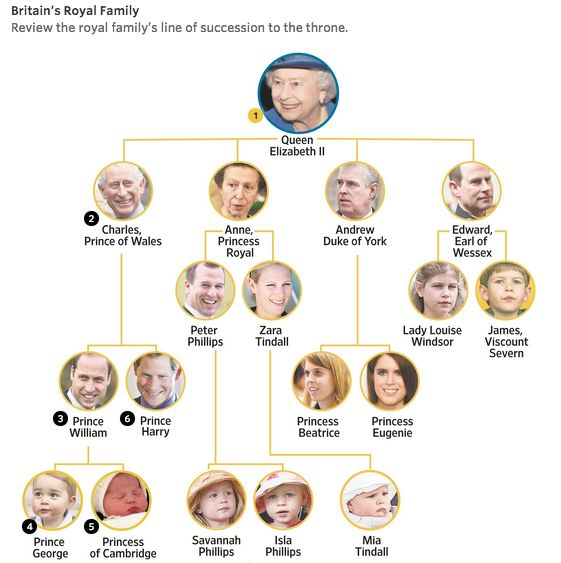
\includegraphics[width=0.6\textwidth]{BritiansRoyalFamily.jpg}
        \caption{Britain's Royal Family}
        \label{fig:family}
    \end{figure}
    \clearpage
    
    \question[2] Using the tree shown in Figure \ref{fig:family}, how many nodes would depth-first-search visit in finding Mia Tindall (including her node)? Assuming we search left-to-right and top-down.

    \textbf{Select one:}
    \begin{checkboxes}
        \choice 3
        \choice 12
        \choice 15
        \choice 18
    \end{checkboxes}

    
    %\clearpage
    \begin{figure}[H]
        \centering
        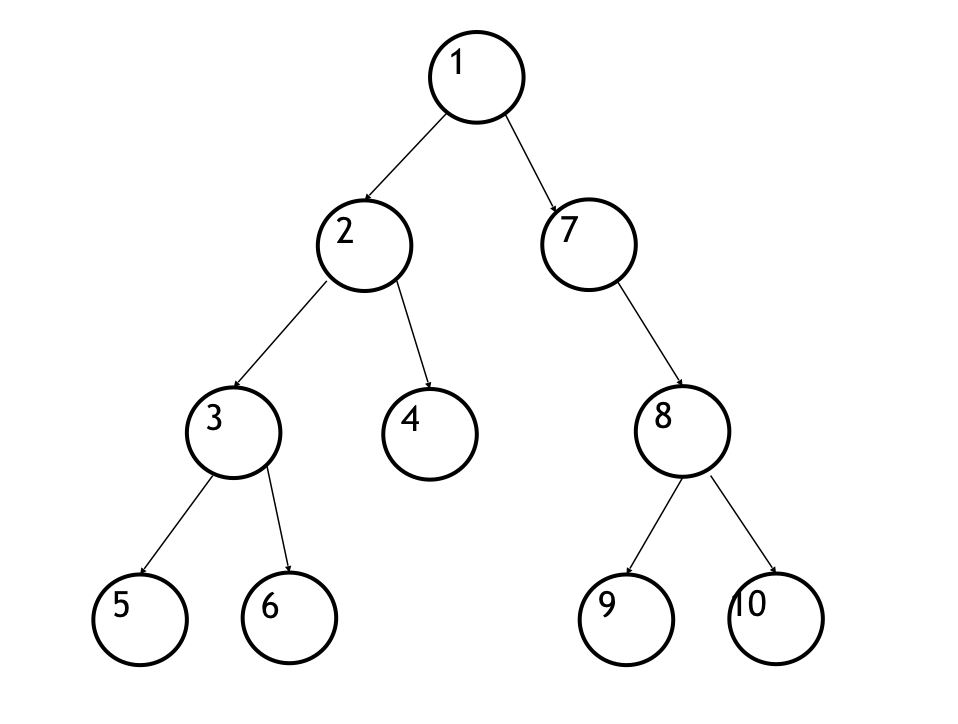
\includegraphics[width = 0.4\textwidth]{TreePlot.png}
        \caption{A Binary Tree with indexed nodes}
        \label{tree}
    \end{figure}
    
    \question[2] Figure \ref{tree} is a Binary Tree with indexed nodes. Assume root node is node 1. What is the node-visit order of \textbf{DFS} and \textbf{BFS} of the above Binary Tree? 
    
    A depth-first search (DFS) traversal of a binary tree starts with visiting the root node, and recursively searches down the left subtree (i.e., the tree rooted at the left node) before going to search the right subtree (i.e., the tree rooted at the right node) until the traversal is done.\\
    Note: Alternatively, we can also look right subtree before left subtree too, for the question please consider left to right order!
    
    A breadth-first search (BFS) traversal of a binary tree visits every node (assuming a left-to-right order) on a level (with the same distance to the root) before going to a lower level until the traversal is done.
    
    The node-visit order of DFS is:
    
    \begin{tcolorbox}[fit,height=1cm, width=\textwidth, blank, borderline={1pt}{-2pt},nobeforeafter]
    %solution
    \end{tcolorbox}
    
    The node-visit order of BFS is:
    
    \begin{tcolorbox}[fit,height=1cm, width=\textwidth, blank, borderline={1pt}{-2pt},nobeforeafter]
    %solution
    \end{tcolorbox}
    
    
    \clearpage
    
    \question[2] Fill in the blanks in the pseudo code for key search using recursive depth-first search (DFS) traversal.
    
    \begin{lstlisting}
    class TreeNode:
        def __init__(self, val):
            self.val = val
            self.leftNode = None
            self.rightNode = None
        
    # (a) the left/right node is denoted as
    #     node.leftNode/node.rightNode
    # (b) left/right node are of type TreeNode
    # (c) the value of the node is denoted as node.val
    # (d) recursive DFS to search for the node 
    #     with value key in a binary tree
    # (e) the left node is assumed to be searched 
    #     before the right node
        
    def find_val(node, key):
        if node is None:
            return None
            
        if (1)____________________________:
            return node
            
        else:
            result = (2)___________________________
            
            if result is None:
                result = (3)___________________________
                
            return (4)___________________________
                
    \end{lstlisting}
    
    \clearpage
    \textbf{\underline{Consider writing a recursive program to solve question 6:}} \\
    Lucas numbers are defined as:
    
    \[ L_n = \begin{cases} 
          2 & \text{if } n = 0\\
          1 & \text{if } n = 1\\
          L_{n-1} + L_{n-2} & \text{if } n > 1
       \end{cases}
    \]
    
    \question[2] Which of the following is the numerical value for $L_{32}$? 

    \textbf{Select one:}
    \begin{checkboxes}
        \choice 3010349
        \choice 3524578
        \choice 4870847
        \choice 7881196
    \end{checkboxes}

    
    \newpage
    \textbf{\underline{Consider the following information to answer questions 7-8:}} \\
    Given the functions of computing a fibonacci number:
    \begin{lstlisting}
    def fib_1(n):
        if n == 0 or n == 1:
            return 1
        return fib_1(n - 1) + fib_1(n - 2)
        
    d = {}
    d[0] = 1
    d[1] = 1
    def fib_2(n):
        if n in d.keys():
            return d[n]
        d[n] = fib_2(n - 1) + fib_2(n - 2)
        return d[n]
        
    \end{lstlisting}
    
    \question[2] Which of the following is the tightest upper bound on the time complexity of computing \lstinline{fib_1(n)}? 

    \textbf{Select one:}
    \begin{checkboxes}
        \choice $O(n)$
        \choice $O(n \log n)$
        \choice $O(2^n)$
        \choice $O(n!)$
    \end{checkboxes}

    
    \question[2] Which of the following is the tightest upper bound on the time complexity of computing \lstinline{fib_2(n)}? 

    \textbf{Select one:}
    \begin{checkboxes}
        \choice $O(n)$
        \choice $O(n \log n)$
        \choice $O(2^n)$
        \choice $O(n!)$
    \end{checkboxes}

    
    
    
    

    \clearpage
\end{questions}

%The following are questions I feel more aligned with the difficulty level of maths encountered in this course
%\input{new_questions.tex}
%\clearpage


\begin{comment} 
{\bf Collaboration Questions} After you have completed all other components of this assignment, report your answers to the collaboration policy questions detailed in the Academic Integrity Policies found \href{http://www.cs.cmu.edu/~mgormley/courses/10601/syllabus.html#7-academic-integrity-policies}{here}.
    \begin{enumerate*}
        \item Did you receive any help whatsoever from anyone in solving this assignment? If so, include full details.
        \item Did you give any help whatsoever to anyone in solving this assignment? If so, include full details?
        \item Did you find or come across code that implements any part of this assignment ? If so, include full details.
    \end{enumerate*}
    
    \begin{tcolorbox}[fit,height=3cm,blank, borderline={1pt}{-2pt},nobeforeafter]
    %Input your solution here.  Do not change any of the specifications of this solution box.
    \end{tcolorbox}
\end{comment}


\textbf{Collaboration Questions} Please answer the following:

\begin{enumerate}
    \item Did you receive any help whatsoever from anyone in solving this assignment? \\Yes / No.
    \begin{itemize}
        \item If you answered `yes', give full details: \_\_\_\_\_\_\_\_\_\_\_\_\_\_\_\_\_\_\_\_
        \item (e.g. “Jane Doe explained to me what is asked in Question 3.4”)
    \end{itemize}
    \item Did you give any help whatsoever to anyone in solving this assignment? \\Yes / No.
    \begin{itemize}
        \item If you answered `yes', give full details: \_\_\_\_\_\_\_\_\_\_\_\_\_\_\_\_\_\_\_\_
        \item (e.g. “I pointed Joe Smith to section 2.3 since he didn’t know how to proceed with Question 2”)
    \end{itemize}
    \item Did you find or come across code that implements any part of this assignment ? \\Yes / No. (See below policy on “found code”)
    \begin{itemize}
        \item If you answered `yes', give full details: \_\_\_\_\_\_\_\_\_\_\_\_\_\_\_\_\_\_\_\_
        \item (book \& page, URL \& location within the page, etc.).
    \end{itemize}
\end{enumerate}

\end{document}